\begin{frame}[fragile]
    \begin{minted}{rust}
let results = b_star(4);

pub fn b_star(n: usize) -> Vec<Queens> {
    let mut results = Vec::new();

    let mut columns = BitVec::from_elem(n, false);
    let mut left_diagonals = BitVec::from_elem(2 * n - 1, false);
    let mut right_diagonals = BitVec::from_elem(2 * n - 1, false);

    let mut rows = Vec::new();
    let mut column = 0;

    // ...
}
    \end{minted}
    $results = [\ ]$\\
    $columns = \raisebox{-2ex}{
\includegraphics[height=\baselineskip * 2]{../img/empty.png}}$ ,
    $left\_diagonals = \raisebox{-2ex}{
\includegraphics[height=\baselineskip * 2]{../img/empty.png}}$,
    $right\_diagonals = \raisebox{-2ex}{
\includegraphics[height=\baselineskip * 2]{../img/empty.png}}$ \\
    $rows = \raisebox{-2ex}{
\includegraphics[height=\baselineskip * 2]{../img/empty.png}}$ \\
    $column = 0$
\end{frame}
\begin{frame}[fragile]
    \begin{minted}[fontsize=\tiny]{rust}
loop {
    while column < n {
        if !(columns[column]
            || left_diagonals[column + rows.len()]
            || right_diagonals[column + n - 1 - rows.len()])
        {
            if rows.len() + 1 < n {
                // <- we are here
                columns.set(column, true);
                left_diagonals.set(column + rows.len(), true);
                right_diagonals.set(column + n - 1 - rows.len(), true);
                rows.push(column);
                column = 0;
            } else {
                // add to results, removed for clarity
            }
        } else {
            column += 1;
        }
    }
    // backtracking, removed for clarity
}
    \end{minted}
    $columns = \raisebox{-2ex}{
\includegraphics[height=\baselineskip * 2]{../img/empty.png}}$ ,
    $left\_diagonals = \raisebox{-2ex}{
\includegraphics[height=\baselineskip * 2]{../img/empty.png}}$,
    $right\_diagonals = \raisebox{-2ex}{
\includegraphics[height=\baselineskip * 2]{../img/empty.png}}$ \\
    $rows = \raisebox{-2ex}{
\includegraphics[height=\baselineskip * 2]{../img/empty.png}}$ \\
    $column = 0$
\end{frame}
\begin{frame}[fragile]
    \begin{minted}[fontsize=\tiny]{rust}
loop {
    while column < n {
        if !(columns[column]
            || left_diagonals[column + rows.len()]
            || right_diagonals[column + n - 1 - rows.len()])
        {
            if rows.len() + 1 < n {
                columns.set(column, true);
                left_diagonals.set(column + rows.len(), true);
                right_diagonals.set(column + n - 1 - rows.len(), true);
                rows.push(column);
                // <- we are here
                column = 0;
            } else {
                // add to results, removed for clarity
            }
        } else {
            column += 1;
        }
    }
    // backtracking, removed for clarity
}
    \end{minted}
    $columns = \raisebox{-2ex}{
\includegraphics[height=\baselineskip * 2]{../img/columns0.png}}$ ,
    $left\_diagonals = \raisebox{-2ex}{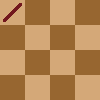
\includegraphics[height=\baselineskip * 2]{../img/left_diagonals0.png}}$,
    $right\_diagonals = \raisebox{-2ex}{
\includegraphics[height=\baselineskip * 2]{../img/right_diagonals3.png}}$ \\
    $rows = \raisebox{-2ex}{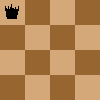
\includegraphics[height=\baselineskip * 2]{../img/state0.png}}$ \\
    $column = 0$
\end{frame}
\begin{frame}[fragile]
    \begin{minted}[fontsize=\tiny]{rust}
loop {
    while column < n {
        if !(columns[column]
            || left_diagonals[column + rows.len()]
            || right_diagonals[column + n - 1 - rows.len()])
        {
            if rows.len() + 1 < n {
                columns.set(column, true);
                left_diagonals.set(column + rows.len(), true);
                right_diagonals.set(column + n - 1 - rows.len(), true);
                rows.push(column);
                column = 0;
            } else {
                // add to results, removed for clarity
            }
        } else {
            column += 1;
            // <- we are here
        }
    }
    // backtracking, removed for clarity
}
    \end{minted}
    $columns = \raisebox{-2ex}{
\includegraphics[height=\baselineskip * 2]{../img/columns0.png}}$ ,
    $left\_diagonals = \raisebox{-2ex}{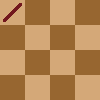
\includegraphics[height=\baselineskip * 2]{../img/left_diagonals0.png}}$,
    $right\_diagonals = \raisebox{-2ex}{
\includegraphics[height=\baselineskip * 2]{../img/right_diagonals3.png}}$ \\
    $rows = \raisebox{-2ex}{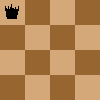
\includegraphics[height=\baselineskip * 2]{../img/state0.png}}$ \\
    $column = 1$
\end{frame}
\begin{frame}[fragile]
    \begin{minted}[fontsize=\tiny]{rust}
loop {
    while column < n {
        if !(columns[column]
            || left_diagonals[column + rows.len()]
            || right_diagonals[column + n - 1 - rows.len()])
        {
            if rows.len() + 1 < n {
                columns.set(column, true);
                left_diagonals.set(column + rows.len(), true);
                right_diagonals.set(column + n - 1 - rows.len(), true);
                rows.push(column);
                column = 0;
            } else {
                // add to results, removed for clarity
            }
        } else {
            column += 1;
            // <- we are here
        }
    }
    // backtracking, removed for clarity
}
    \end{minted}
    $columns = \raisebox{-2ex}{
\includegraphics[height=\baselineskip * 2]{../img/columns0.png}}$ ,
    $left\_diagonals = \raisebox{-2ex}{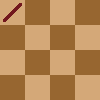
\includegraphics[height=\baselineskip * 2]{../img/left_diagonals0.png}}$,
    $right\_diagonals = \raisebox{-2ex}{
\includegraphics[height=\baselineskip * 2]{../img/right_diagonals3.png}}$ \\
    $rows = \raisebox{-2ex}{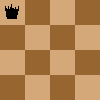
\includegraphics[height=\baselineskip * 2]{../img/state0.png}}$ \\
    $column = 2$
\end{frame}
\begin{frame}[fragile]
    \begin{minted}[fontsize=\tiny]{rust}
loop {
    while column < n {
        if !(columns[column]
            || left_diagonals[column + rows.len()]
            || right_diagonals[column + n - 1 - rows.len()])
        {
            if rows.len() + 1 < n {
                columns.set(column, true);
                left_diagonals.set(column + rows.len(), true);
                right_diagonals.set(column + n - 1 - rows.len(), true);
                rows.push(column);
                column = 0;
                // <- we are here
            } else {
                // add to results, removed for clarity
            }
        } else {
            column += 1; 
        }
    }
    // backtracking, removed for clarity
}
    \end{minted}
    $columns = \raisebox{-2ex}{
\includegraphics[height=\baselineskip * 2]{../img/columns02.png}}$ ,
    $left\_diagonals = \raisebox{-2ex}{
\includegraphics[height=\baselineskip * 2]{../img/left_diagonals03.png}}$,
    $right\_diagonals = \raisebox{-2ex}{
\includegraphics[height=\baselineskip * 2]{../img/right_diagonals34.png}}$ \\
    $rows = \raisebox{-2ex}{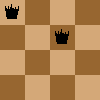
\includegraphics[height=\baselineskip * 2]{../img/state02.png}}$ \\
    $column = 0$
\end{frame}
\begin{frame}[fragile]
    \begin{minted}[fontsize=\tiny]{rust}
loop {
    // while ...
    
    // <- we are here
    if let Some(prev) = rows.pop() {
        right_diagonals.set(prev + n - 1 - rows.len(), false);
        left_diagonals.set(prev + rows.len(), false);
        columns.set(prev, false);
        column = prev + 1;
    } else {
        break;
    }
}
    \end{minted}
    $columns = \raisebox{-2ex}{
\includegraphics[height=\baselineskip * 2]{../img/columns02.png}}$ ,
    $left\_diagonals = \raisebox{-2ex}{
\includegraphics[height=\baselineskip * 2]{../img/left_diagonals03.png}}$,
    $right\_diagonals = \raisebox{-2ex}{
\includegraphics[height=\baselineskip * 2]{../img/right_diagonals34.png}}$ \\
    $rows = \raisebox{-2ex}{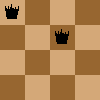
\includegraphics[height=\baselineskip * 2]{../img/state02.png}}$ \\
    $column = 4$
\end{frame}
\begin{frame}[fragile]
    \begin{minted}[fontsize=\tiny]{rust}
loop {
    // while ...
    
    if let Some(prev) = rows.pop() {
        right_diagonals.set(prev + n - 1 - rows.len(), false);
        left_diagonals.set(prev + rows.len(), false);
        columns.set(prev, false);
        column = prev + 1;
        // <- we are here
    } else {
        return results;
    }
}
    \end{minted}
    $prev = 2$\\
    $columns = \raisebox{-2ex}{
\includegraphics[height=\baselineskip * 2]{../img/columns0.png}}$ ,
    $left\_diagonals = \raisebox{-2ex}{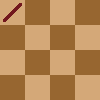
\includegraphics[height=\baselineskip * 2]{../img/left_diagonals0.png}}$,
    $right\_diagonals = \raisebox{-2ex}{
\includegraphics[height=\baselineskip * 2]{../img/right_diagonals3.png}}$ \\
    $rows = \raisebox{-2ex}{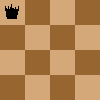
\includegraphics[height=\baselineskip * 2]{../img/state0.png}}$ \\
    $column = 3$
\end{frame}
\begin{frame}[fragile]
    \begin{minted}[fontsize=\tiny]{rust}
loop {
    while column < n {
        if !(columns[column]
            || left_diagonals[column + rows.len()]
            || right_diagonals[column + n - 1 - rows.len()])
        {
            if rows.len() + 1 < n {
                // update rows etc, removed for clarity
            } else {
                // <- we are here
                let mut q = rows.clone();
                q.push(column);
                results.push(Queens { n, rows: q });
                column += 1;
            }
        } else {
            column += 1; 
        }
    }
    // backtracking, removed for clarity
}
    \end{minted}
    $columns = \raisebox{-2ex}{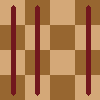
\includegraphics[height=\baselineskip * 2]{../img/columns013.png}}$ ,
    $left\_diagonals = \raisebox{-2ex}{
\includegraphics[height=\baselineskip * 2]{../img/left_diagonals124.png}}$,
    $right\_diagonals = \raisebox{-2ex}{
\includegraphics[height=\baselineskip * 2]{../img/right_diagonals145.png}}$ \\
    $rows = \raisebox{-2ex}{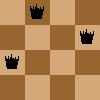
\includegraphics[height=\baselineskip * 2]{../img/state130.png}}$ \\
    $column = 2$
\end{frame}
\begin{frame}[fragile]
    \begin{minted}[fontsize=\tiny]{rust}
loop {
    while column < n {
        if !(columns[column]
            || left_diagonals[column + rows.len()]
            || right_diagonals[column + n - 1 - rows.len()])
        {
            if rows.len() + 1 < n {
                // update rows etc, removed for clarity
            } else {
                let mut q = rows.clone();
                q.push(column);
                results.push(Queens { n, rows: q });
                column += 1;
                // <- we are here
            }
        } else {
            column += 1; 
        }
    }
    // backtracking, removed for clarity
}
    \end{minted}
    $results = [\raisebox{-2ex}{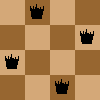
\includegraphics[height=\baselineskip * 2]{../img/state1302.png}}]$ \\
    $rows = \raisebox{-2ex}{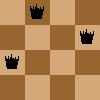
\includegraphics[height=\baselineskip * 2]{../img/state130.png}}$ \\
    $column = 3$
\end{frame}
\begin{frame}[fragile]
    \begin{minted}[fontsize=\tiny]{rust}
loop {
    // while ...
    
    // <- we are here
    if let Some(prev) = rows.pop() {
        right_diagonals.set(prev + n - 1 - rows.len(), false);
        left_diagonals.set(prev + rows.len(), false);
        columns.set(prev, false);
        column = prev + 1;    
    } else {
        return results;
    }
}
    \end{minted}
    $columns = \raisebox{-2ex}{
\includegraphics[height=\baselineskip * 2]{../img/empty.png}}$ ,
    $left\_diagonals = \raisebox{-2ex}{
\includegraphics[height=\baselineskip * 2]{../img/empty.png}}$,
    $right\_diagonals = \raisebox{-2ex}{
\includegraphics[height=\baselineskip * 2]{../img/empty.png}}$ \\
    $rows = \raisebox{-2ex}{
\includegraphics[height=\baselineskip * 2]{../img/empty.png}}$ \\
    $column = 4$
    $results = [
    \raisebox{-2ex}{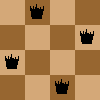
\includegraphics[height=\baselineskip * 2]{../img/state1302.png}},
    \raisebox{-2ex}{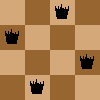
\includegraphics[height=\baselineskip * 2]{../img/state2031.png}}
    ]$
\end{frame}